% This file is part of the Apogee project.
% Copyright 2014 Melissa Ness and David W. Hogg.

\documentclass[12pt, preprint]{aastex}

\newcommand{\teff}{\mbox{$\rm T_{eff}$}}
\newcommand{\feh}{\mbox{$\rm [Fe/H]$}}
\newcommand{\logg}{\mbox{$\rm \log g$}}

\begin{document}



\section{Introduction}

Challenges of stellar parameter estimation.

In principle there could be data-driven models.

Data-driven models would permit ``label transfer''.
This is especially important if we want optical models to provide labels for infrared surveys (and so on).

APOGEE provides a great data set for exploring these issues. Large homogenous datasets make this possible for the first time. 

Also avoids issue of stellar models once have well characterised set, given any wavelength for calibration and is very fast + generalised. 
issues - cite Meszaros paper for typical implementation. 

We implement this technique as a method to systematically and optimally exploit the information in stellar spectra within large homogeneous datasets.  Our method avoids explicit stellar models and the data itself is the basis of the characterisation. Models are required ab initio and can be implemented at an independent wavelength range, to set the labels for the calibration data.  We apply the primary spectral labels of \teff\, \logg\, [Fe/H] and this process can be extended and applied in N dimensions given well labeled training sets. Calibration sets, of open and globular cluster data, are critical to enable this method which can in principle be implemented with synthetic libraries but this folds in unphysical residuals. We present a general method by using the APOGEE example, characterising the APOGEE spectra and demonstrating how dimensionality of the calibration set can be applied to interpret APOGEE data. 

Motivated by the idea of fingerprinting spectra in the spirt of chemical tagging and developing robust methods that allow the spectra to be mapped in full as a function of its labels. Reverse philosophy to a lot of current techniques were individual lines are the focus, here we disregard what they are and examine impartially. This may reveal information that may not be obvious or otherwise determined. note - Can I find an example of this for the paper? 

%map labels of test set onto the larger set of data

\section{Motivation}

Proof-of-concept: 

We identified a number of regions in APOGEE spectra that serve as relatively temperature and log g insensitive metallicity indicators that can be used to return an [Fe/H] for APOGEE spectra to an accuracy of $<$ 0.15 dex. From this first proof-of-concept phase, we have implemented a regression analysis in pixel or line space, to determine the coefficients or spectral regions that might serve as stellar parameter indicators.  We have a number of aims: (i) characterise the dependence of each pixel on the stellar parameters and identify the key regions of the spectra that are sensitive to the stellar parameters we wish to determine (Teff, log g, [Fe/H], [alpha/Fe]), (ii) use the fits to these regions (using calibration stars) as a baseline to derive the stellar parameters from any given APOGEE spectra and (iii) provide a tool to the community for implementation in the APOGEE-2 project + e.g. Hermes, where stellar parameters can be determined without explicit stellar models. Extensions of this are for individual abundance labels and heuristic index determination.\\

\section{Data}

read in data; which files, etc.

re-continuum-normalize; how?

demonstrate that the normalization is good.

meta-data on cluster stars; why do we believe it; table

\section{Spectral model}

linear model plus scatter.

Subtract off and save mean values of meta-data.

likelihood function.

implementation and outputs, figures.

is this a good model?

\section{Parameter estimation}

we want to label other stars

index concept

spectral fitting concept

methodological details

leave-one-out cross-validation on the training spectra

leave-one-cluster-out cross-validation

application to some example APOGEE targets

comparison to ASPCAP

\section{Discussion}

Did it work and etc?

Limitations of the training sample.

Linear model is a very rigid assumption; obviously wrong.
Generalize to a GP at every wavelength.

Applications, esp chemical tagging

\section{Draft Figures}


\begin{figure}[h!]
  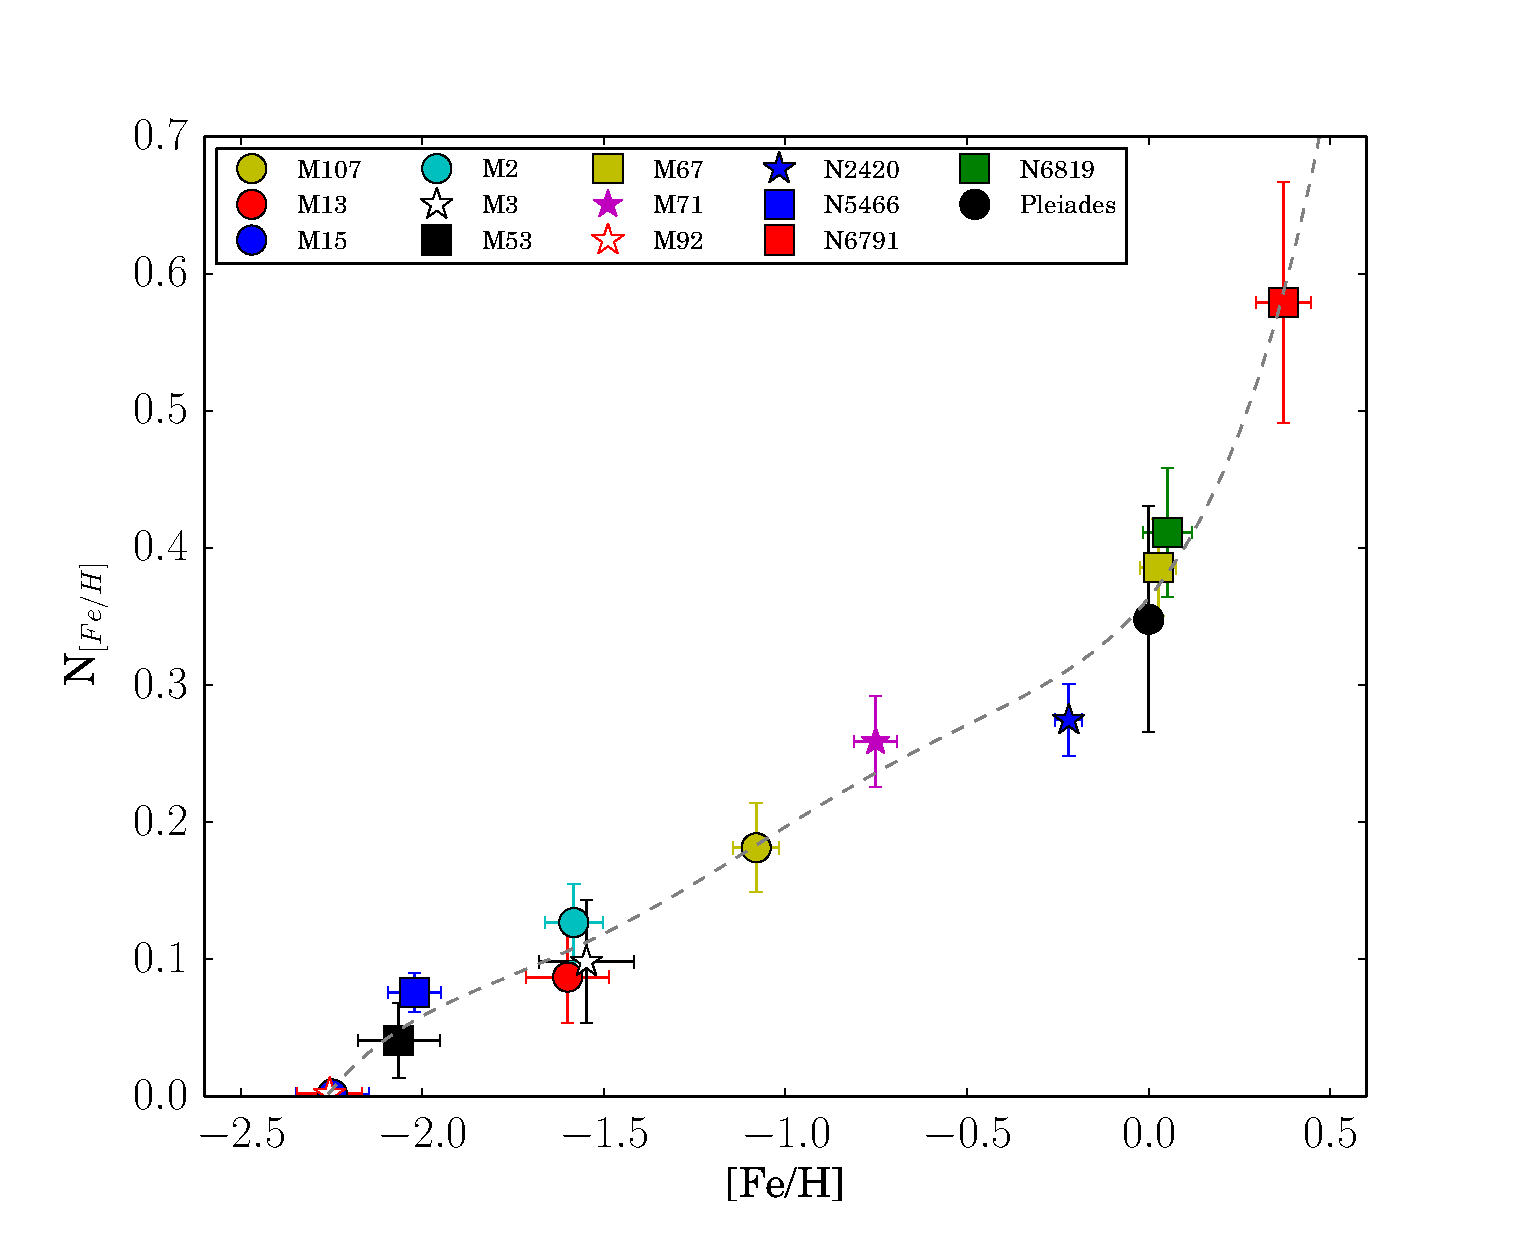
\includegraphics[width=\hsize]{./plots/metals_index.eps}
\caption{Proof of concept/motivating background: The calibration of metallicity of the clusters using an index N$_{[Fe/H]}$, derived from 30 $\AA$ (1\%) of the spectra, using 5 $\times$ lines determined to be [Fe/H]-sensitive and relatively \logg\ and \teff\ insensitive. The error bars represent the dispersion of the points
  around the mean. In total about 450  stars have been used for this
  calibration: M~107 (18 stars), M~13 (71 stars), M~15 (11 stars), M~2
  (19 stars), M~3 (73 stars), M~53 (16 stars), M~67 (24 stars), M~71
  (6 stars), M~92 (48 stars), NGC~2420 (9 stars), NGC~5466 (8 stars),
  NGC~6791 (23 stars), NGC~6819 (29 stars), and Pleiades (75 stars)  \textbf{Note I am missing some clusters in this I should add them in} .}
\label{fig:index}
\end{figure}

\begin{figure}[h!]
  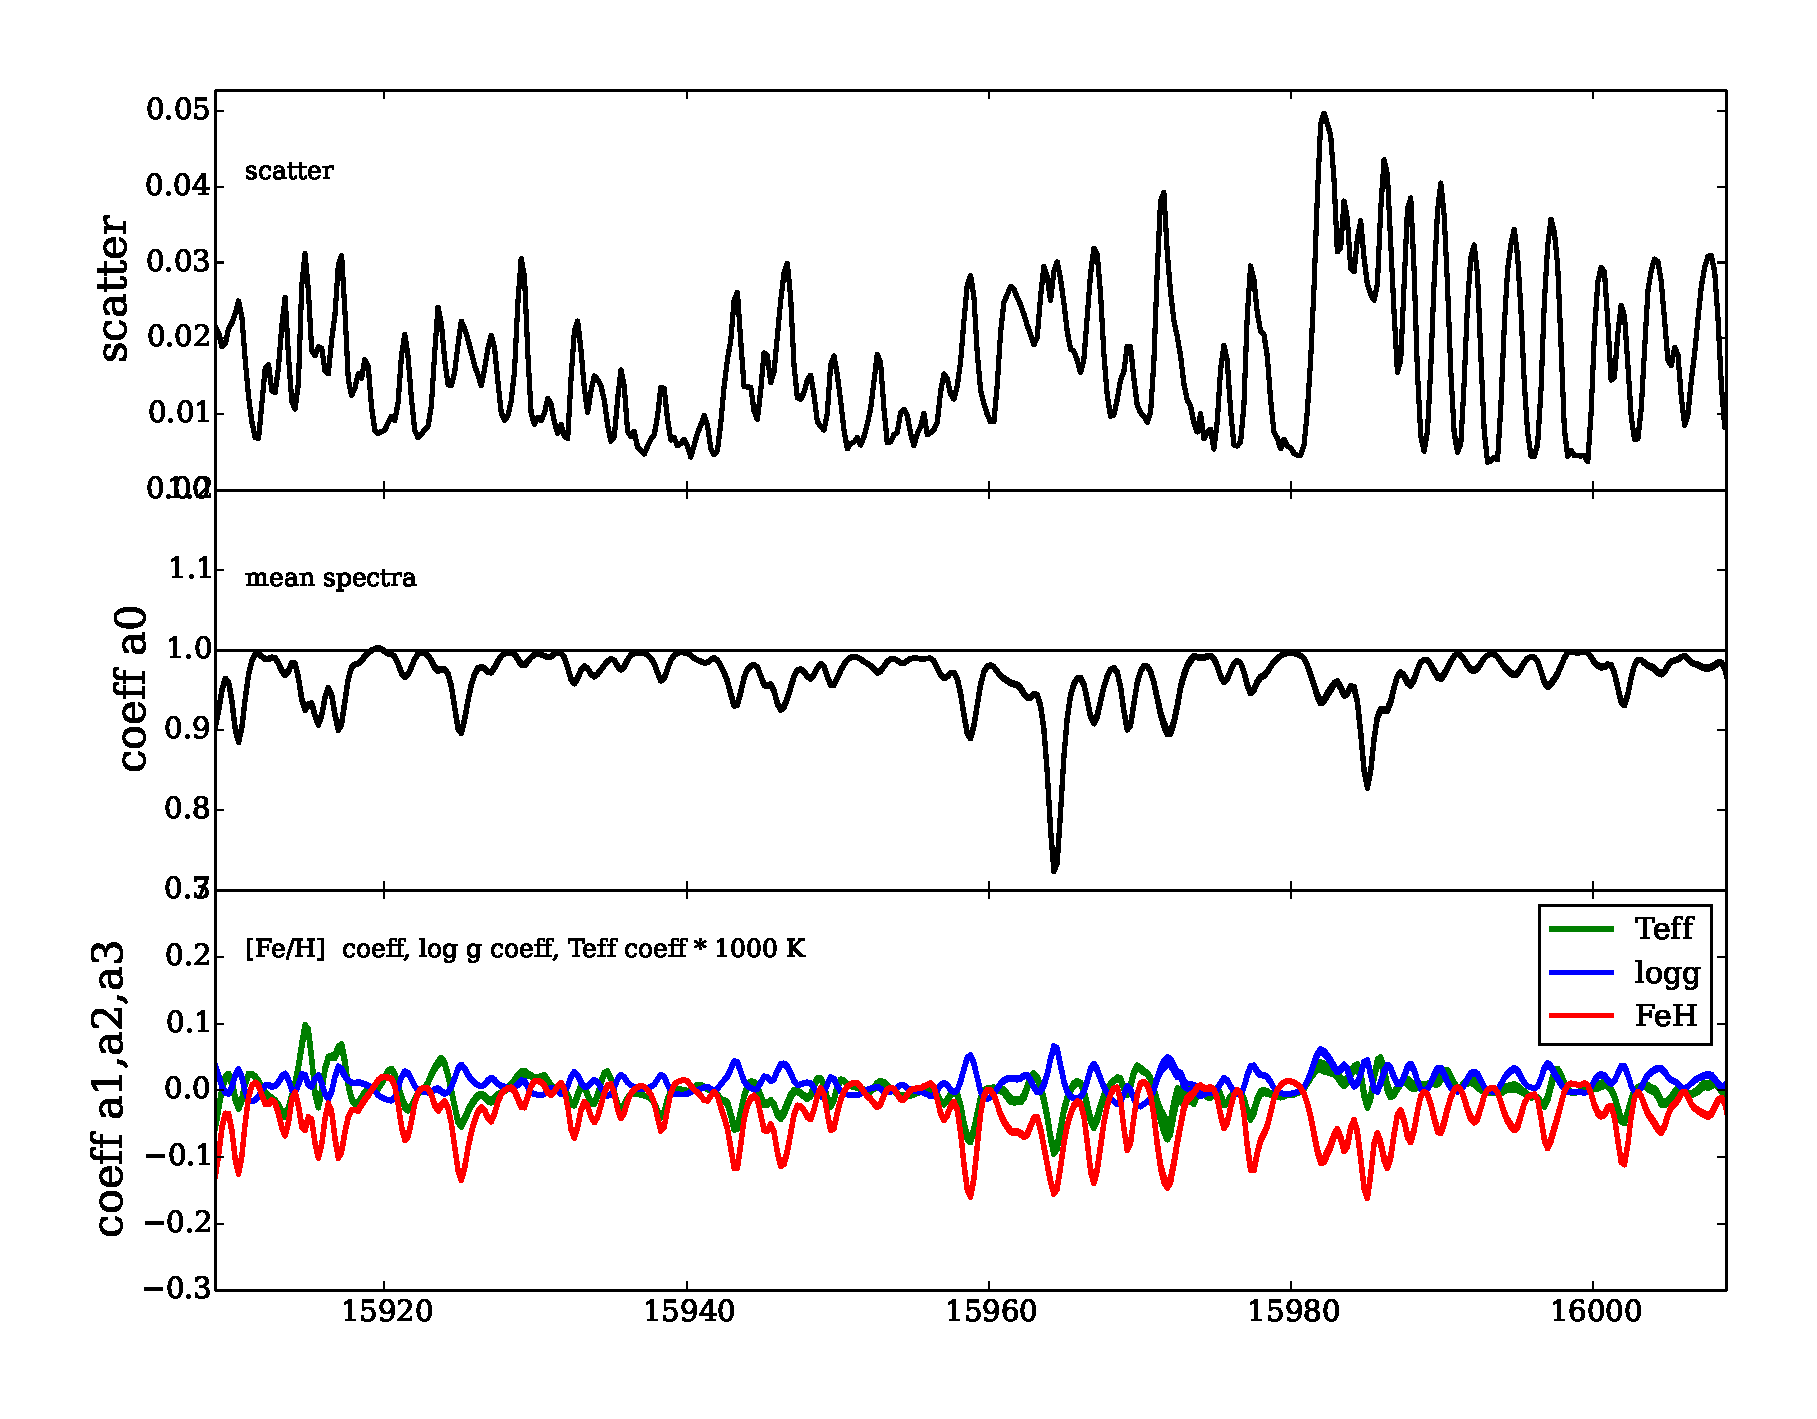
\includegraphics[width=\hsize]{./plots/R1_example.eps}
\caption{The results from the linear regression across at 100 $\AA$ sample region of spectra. The top panel shows the scatter at each wavelength, the centre panel shows the mean spectrum derived from the training set and the bottom panel shows the coefficients fit in each dimension, \teff\, \logg\, [Fe/H]. Given additional labels it will be possible to include more dimensionality, for example [$\alpha$/Fe] and [X/Fe].}
\label{fig:fits}
\end{figure}

\begin{figure}[h!]
  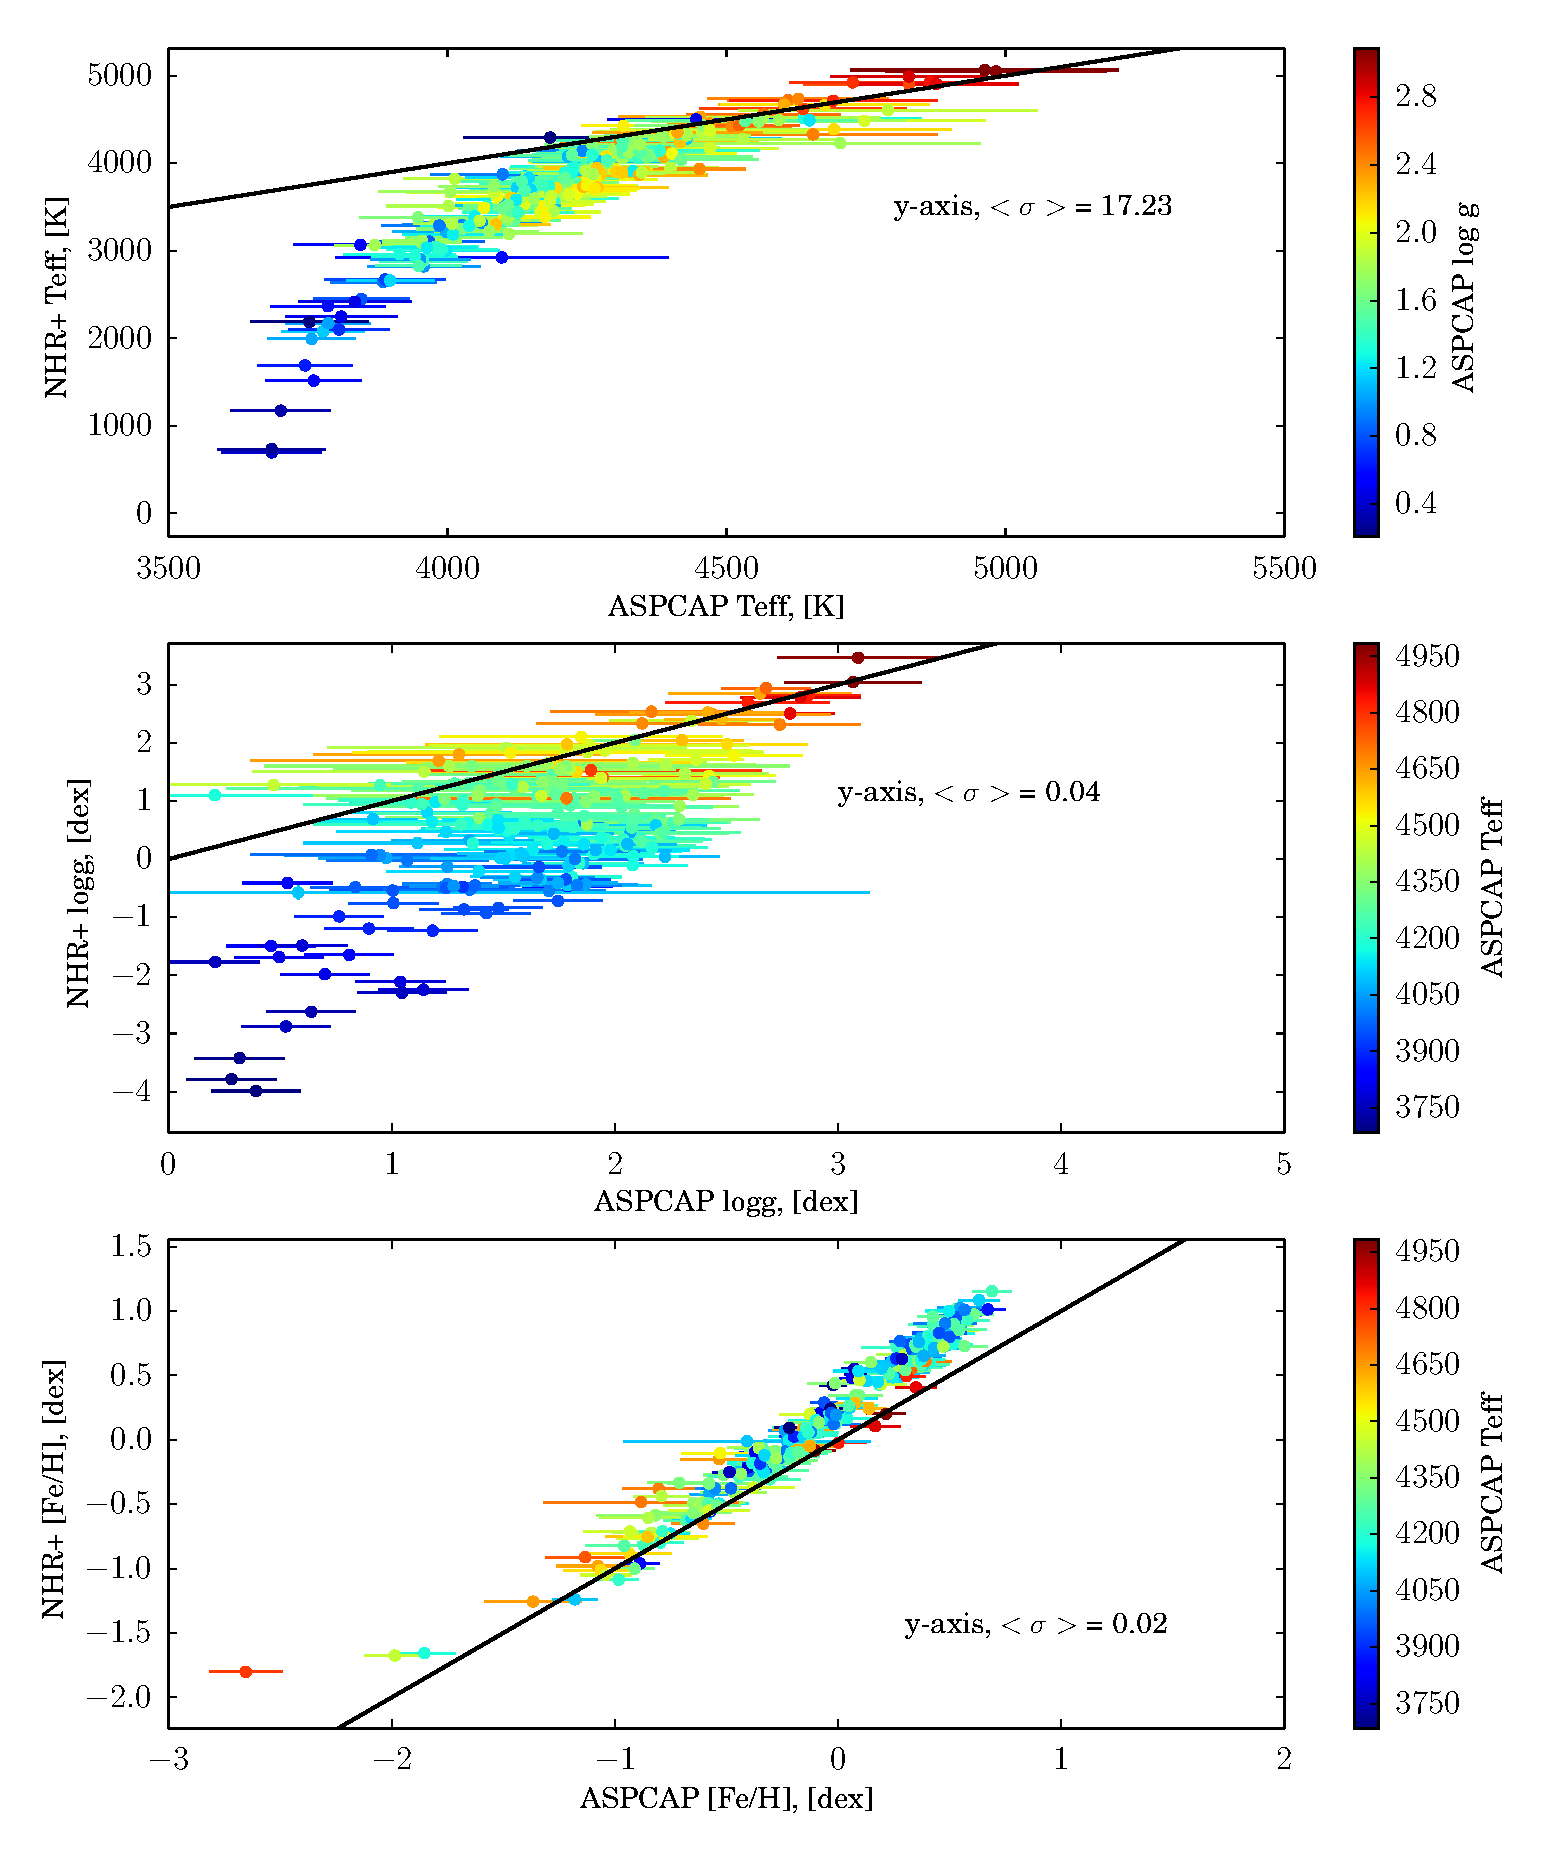
\includegraphics[width=\hsize]{./plots/fits_all3.eps}
\caption{\small{Comparison of our method with ASCAP results for the field 4332 (l,b) = (0,-5$^\circ$). The tight correlation in \teff\ and [Fe/H] suggests that these labels in the training set are very good. There is more scatter in the \logg\ panel that may not represent bad labels in the training set and therefore may not be accounted for in the non-linear model. Comparing Figure \ref{fig:index} with the bottom panel, the discontinuity at ASCAP [Fe/H] $\sim$ 0, is due to the non-linear behaviour of the [Fe/H] which is seen in the index, but which is not captured in our linear model (see Figure \ref{fig:index}).}}
\label{fig:cal}
\end{figure}

\begin{figure}[h!]
  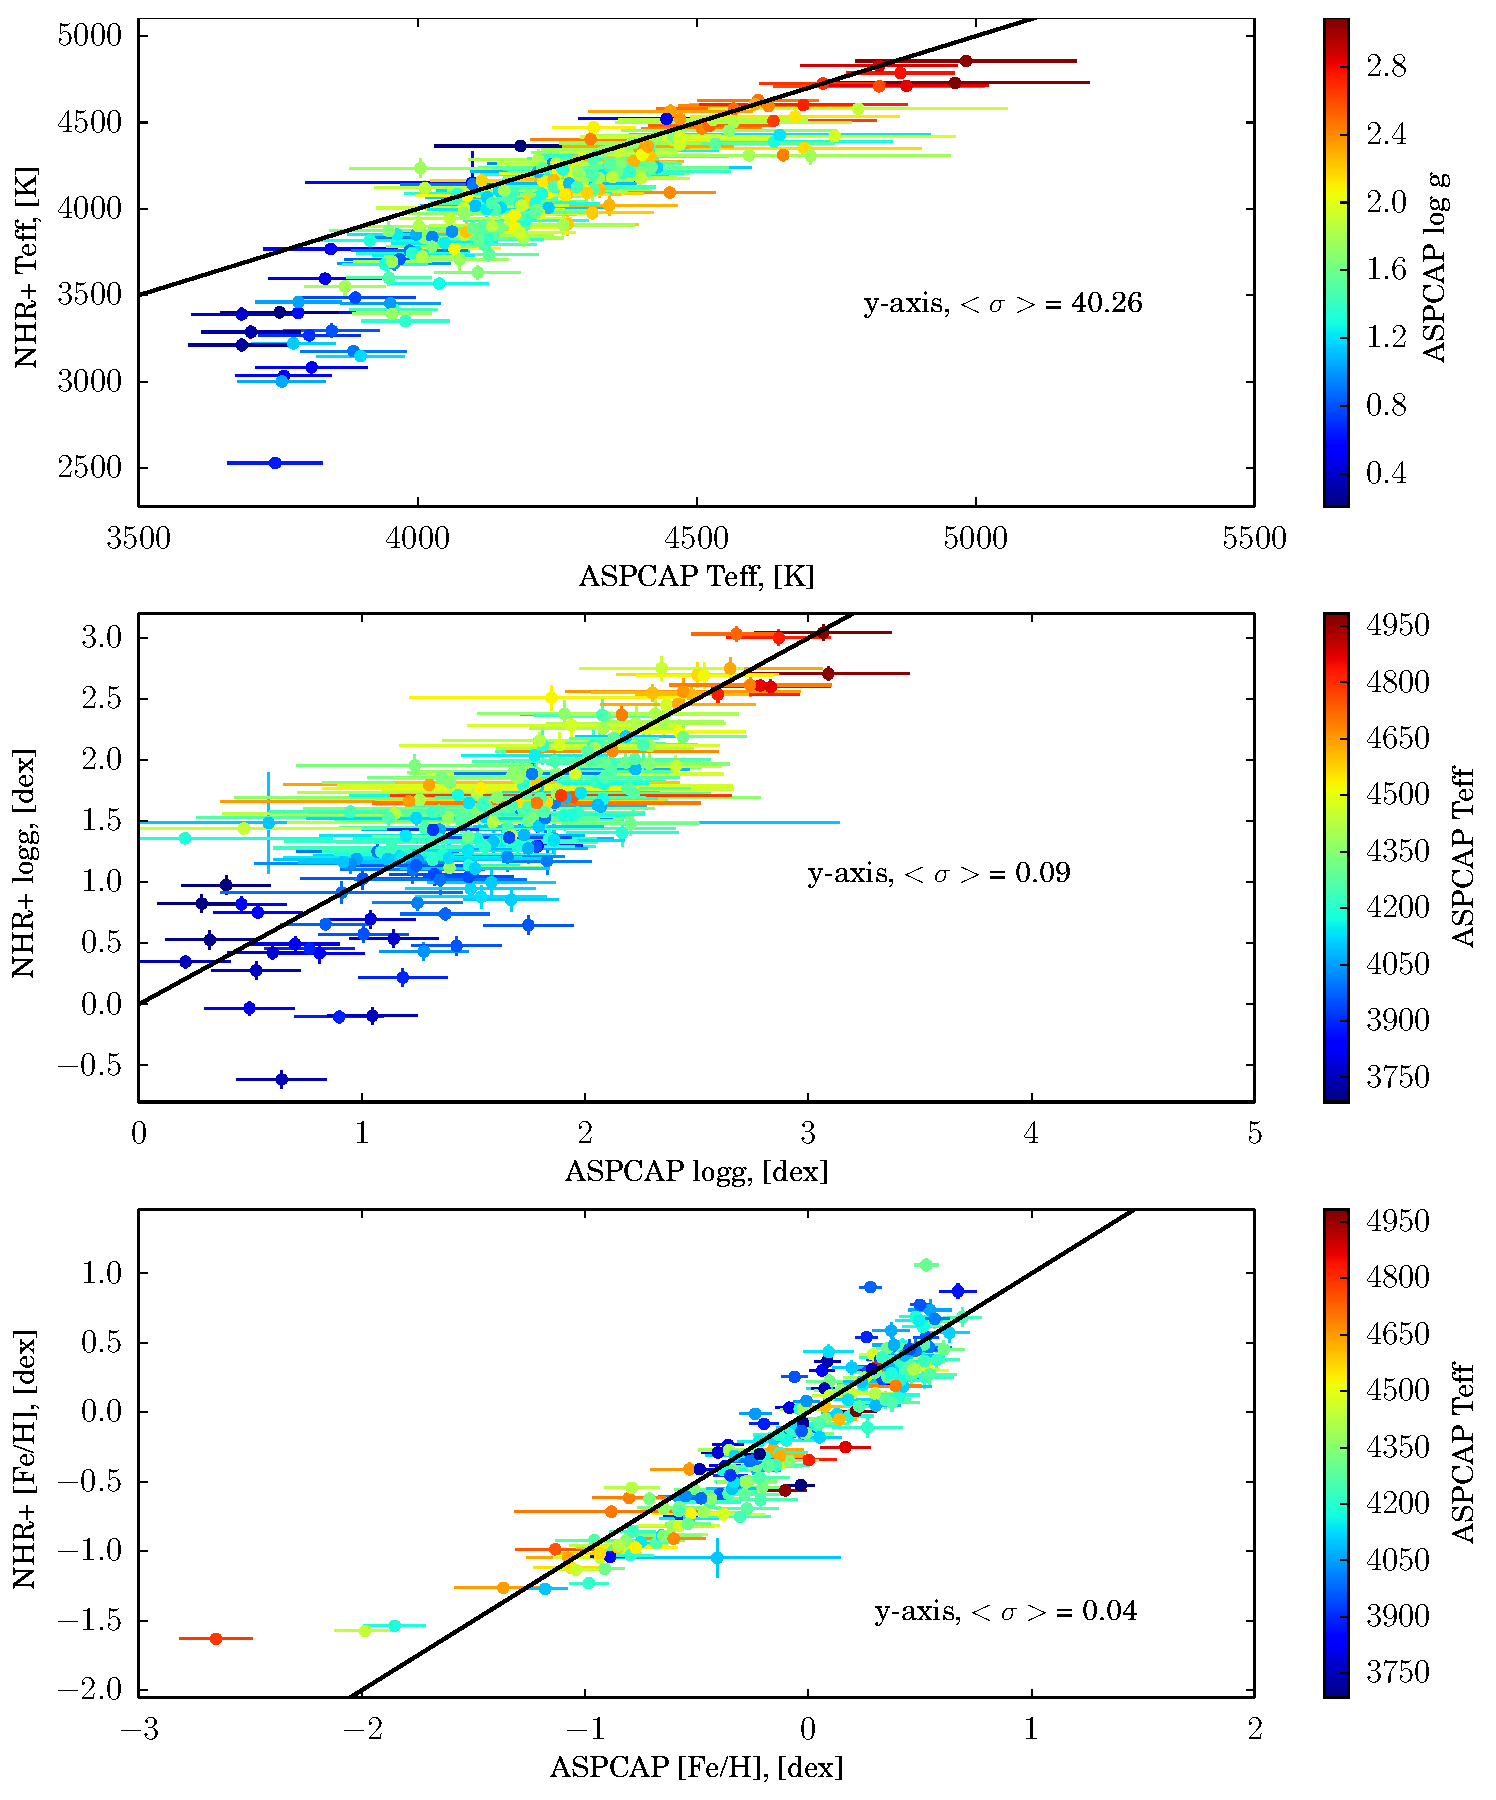
\includegraphics[width=\hsize]{./plots/fits_all3_continuumcut.eps}
\caption{\small{Comparison of our method with ASCAP results for the field 4332, using a continuum cut to select for the weak features and to exclude stronger lines. This was done to avoid the known effect of non-linearities in stronger absorption features and the cut implemented for this figure is 0.935 $<$ flux $<$ 0.99, equivalent to about 50\% of the flux of the median spectra. (note: both bounds are necessary to achieve these fits). Using weaker lines, a linear model is demonstrated to be a reasonably good model for the data. The scatter increases by about a factor of 2 in each dimension by adopting this continuum cut. }}
\label{fig:cut1}
\end{figure}

\begin{figure}[h!]
  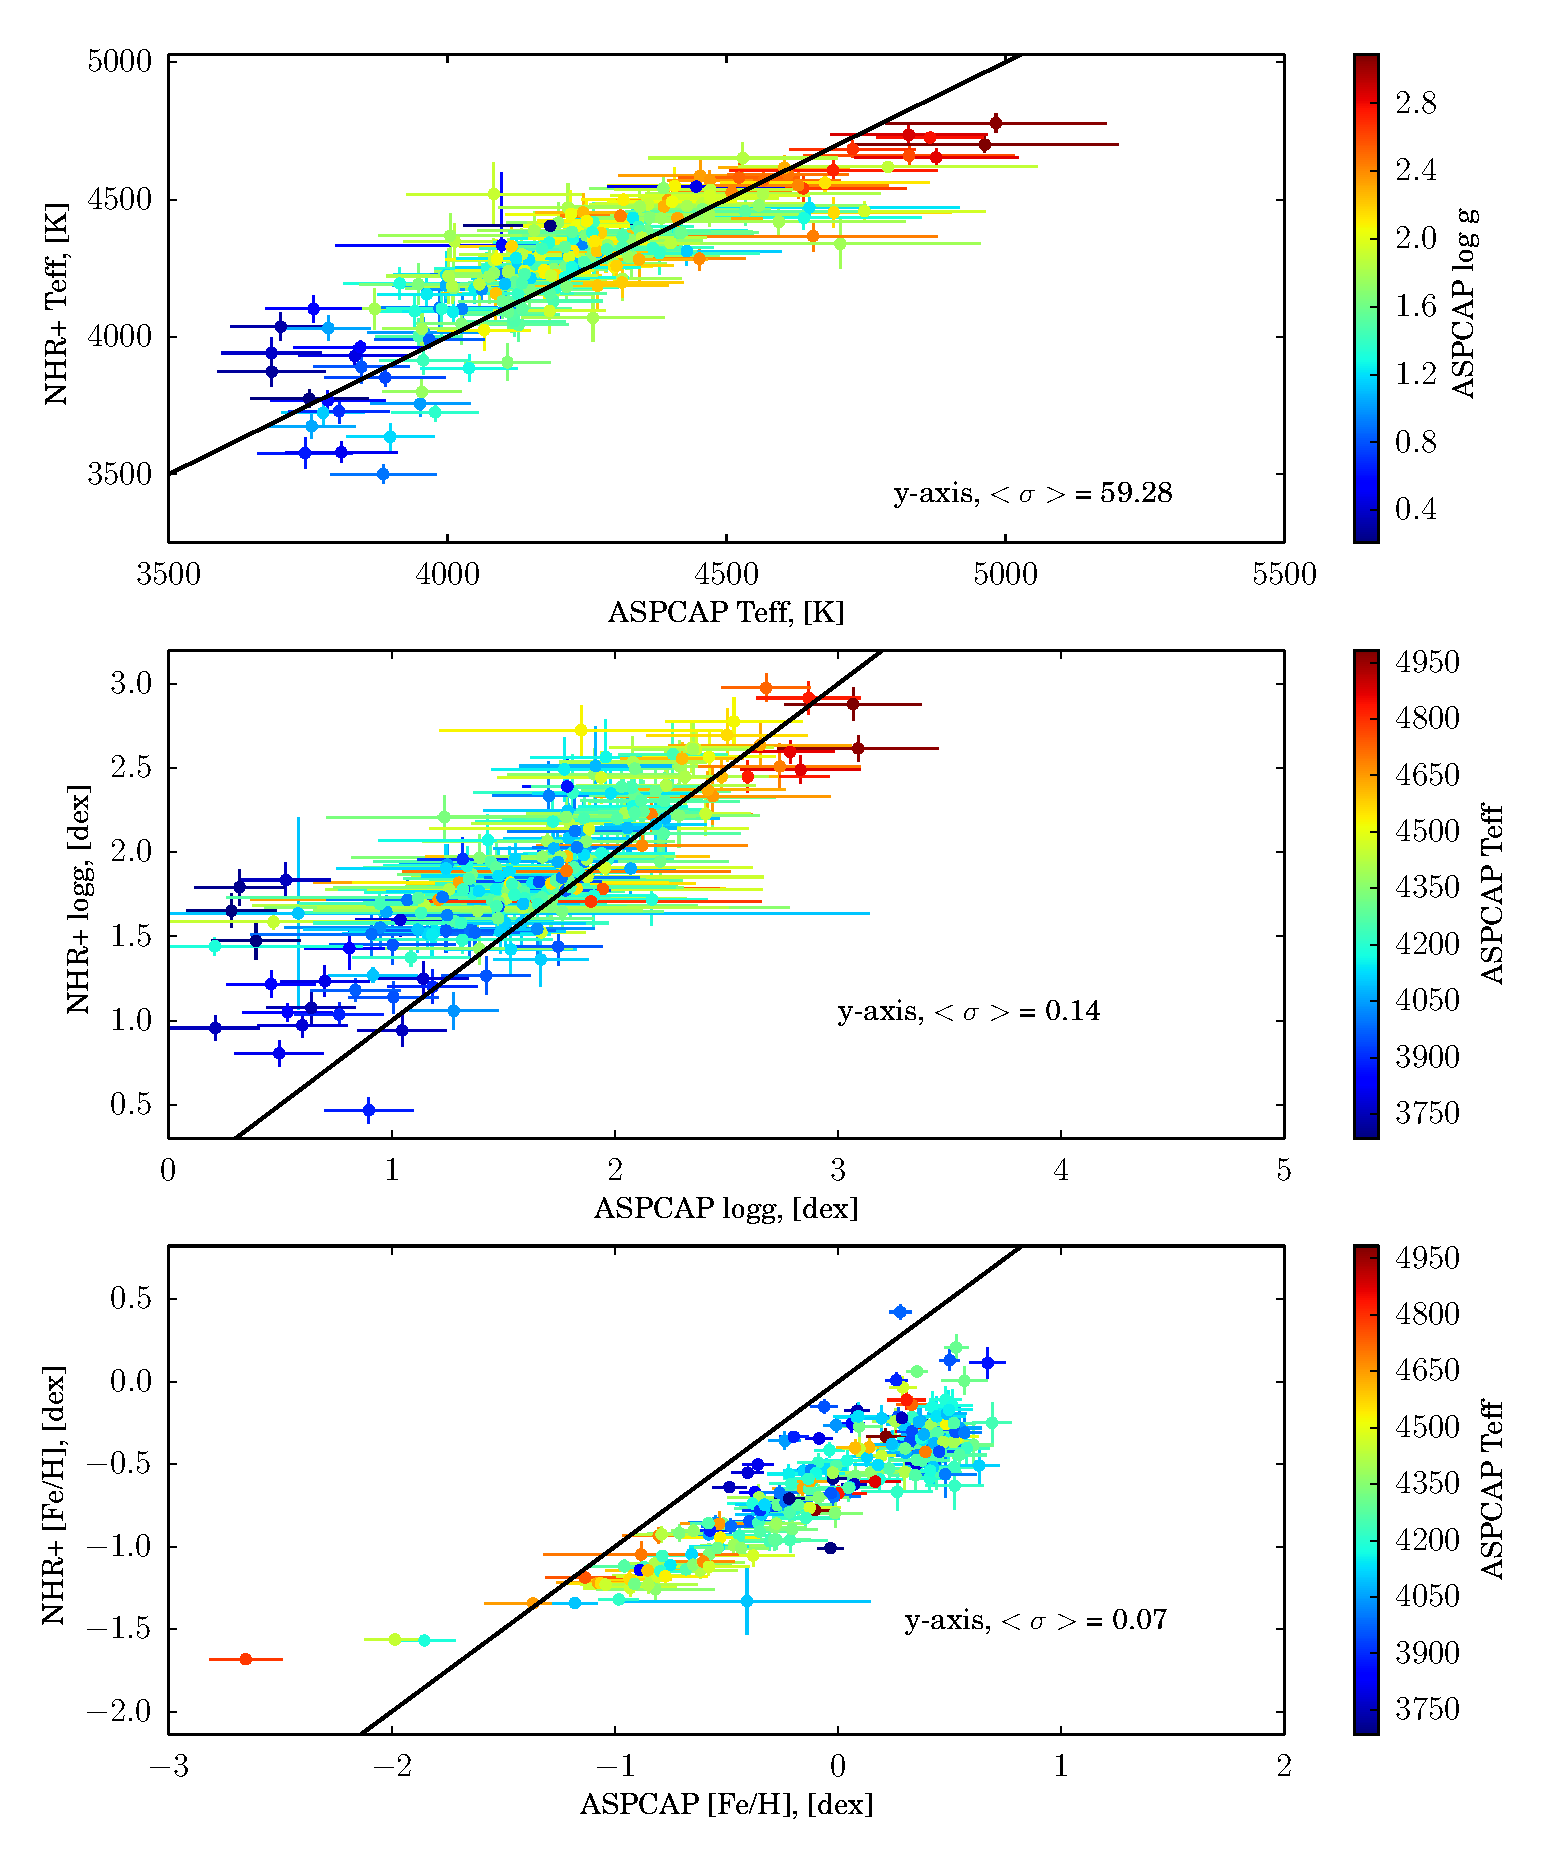
\includegraphics[width=\hsize]{./plots/fits_all3_continuumcut2.eps}
\caption{\small{As for figure \ref{fig:cut1} but using a tighter continuum cut of 0.95 $<$ flux $<$ 0.99. This demonstrates that the information for the [Fe/H] characterisation is lost at this tighter cut on the continuum, it suggests that the sensitivity of the spectra to log g is lower at the low temperature end of the spectra and the information in temperature is fairly well recovered using a linear scale for this cut in flux. } }
\label{fig:cut2}
\end{figure}

\begin{figure}[h!]
  \includegraphics[width=\hsize]{./plots/coeff_map.eps}
\caption{per pixel scaled residuals for stars ordered in [Fe/H], from the most metal poor at the bottom to the most metal rich at the top}
\label{fig:coeff}
\end{figure}

\begin{figure}[h!]
  \includegraphics[width=\hsize]{./plots/chi_map.eps}
\caption{Spectral Fingerprints for calibration clusters showing the chi2 coefficients for each star at each pixel separated into clusters from the most metal rich to the most metal poor (divided by horizontal lines) 
\textbf{To do; put clusters + [Fe/H] on other y-axis)}}
\label{fig:DNA}
\end{figure}

\begin{figure}[h!]
  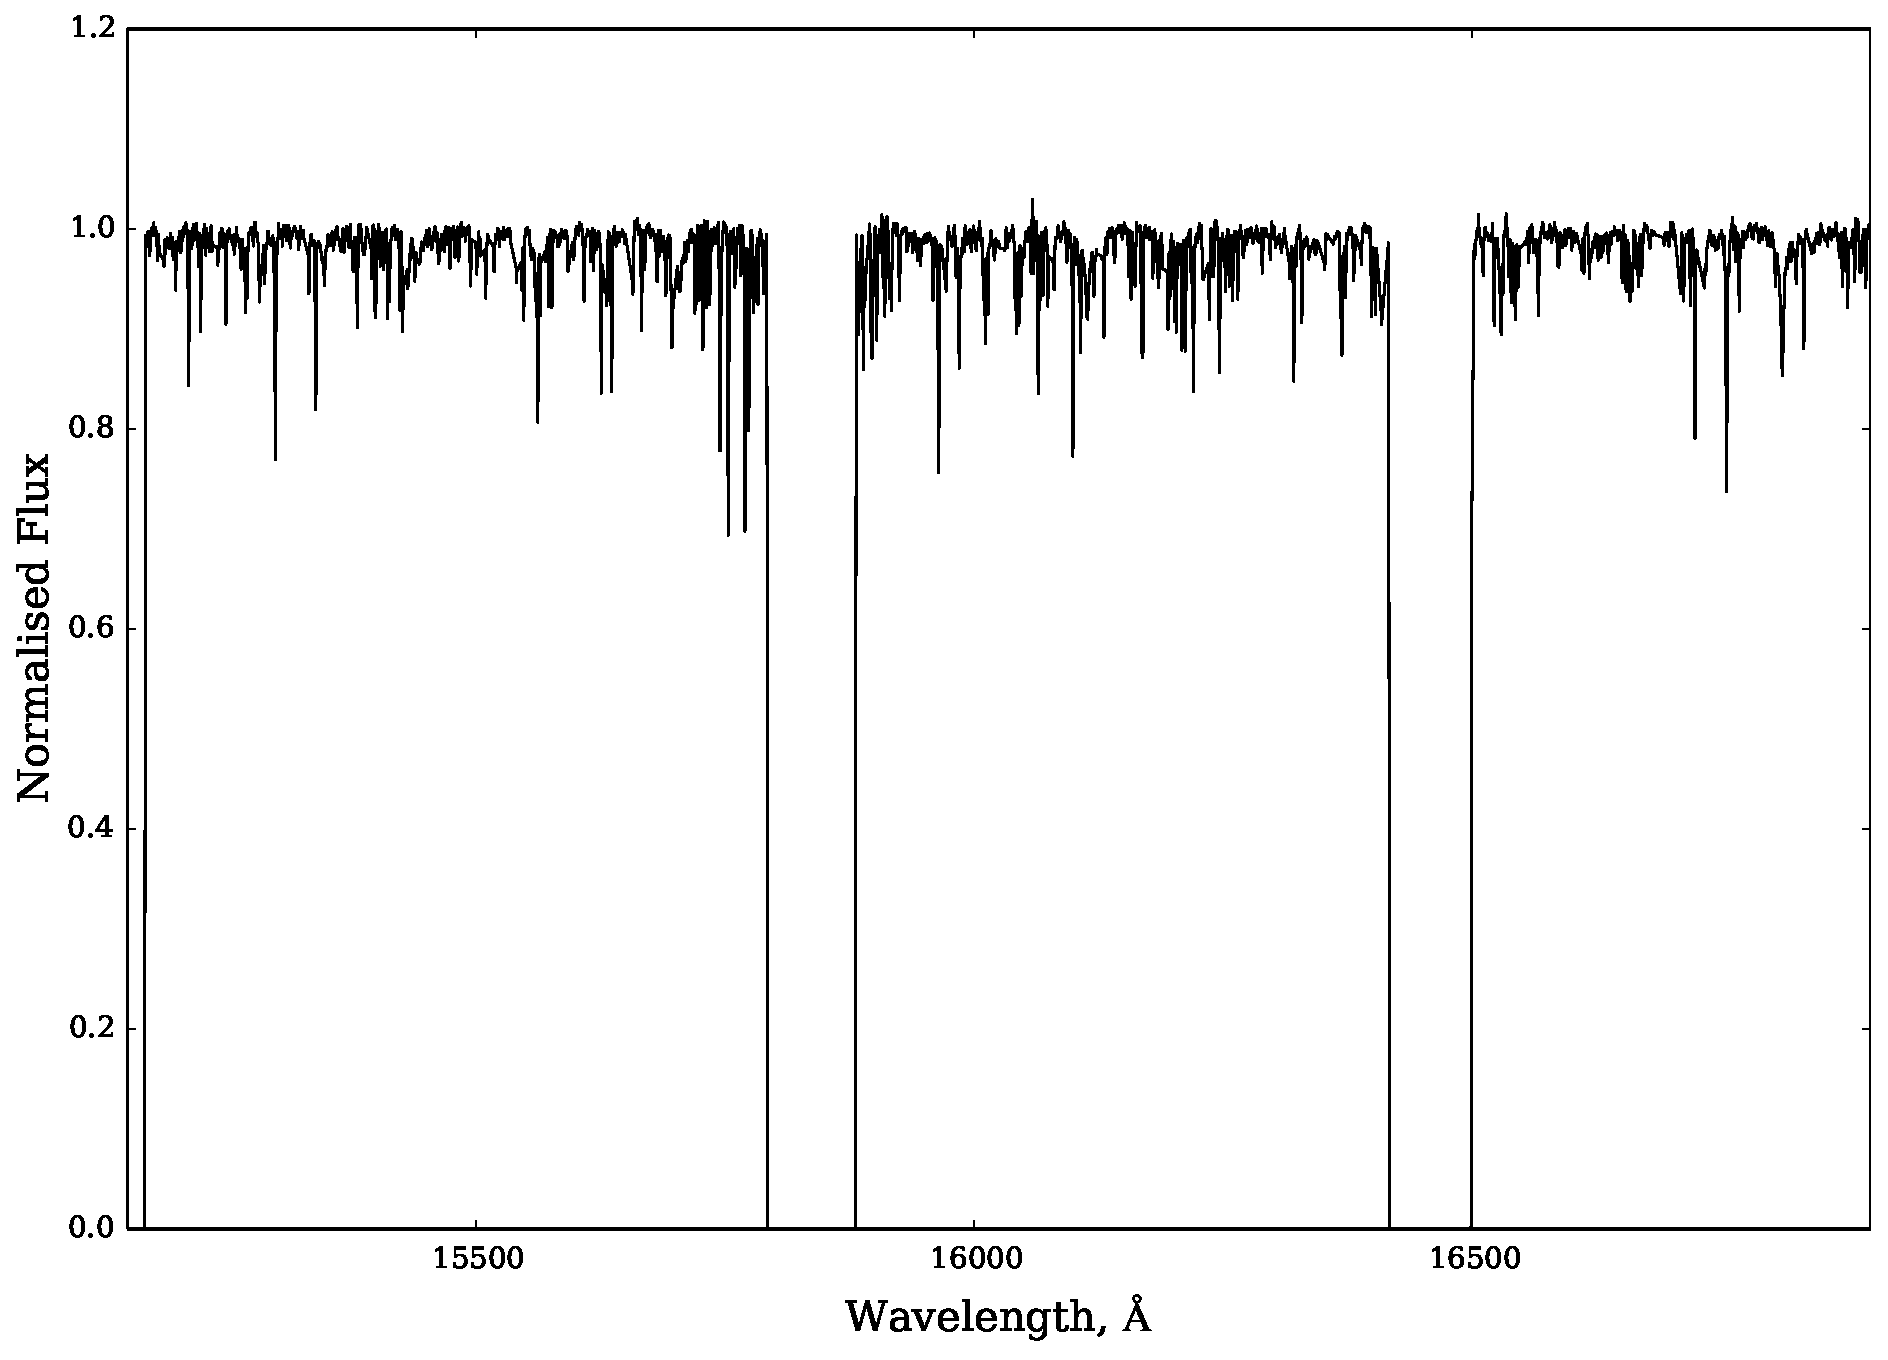
\includegraphics[width=\hsize]{./plots/normed_300.eps}
\caption{Sample continuum normalised spectra}
\label{fig:DNA}
\end{figure}

\begin{figure}[h!]
  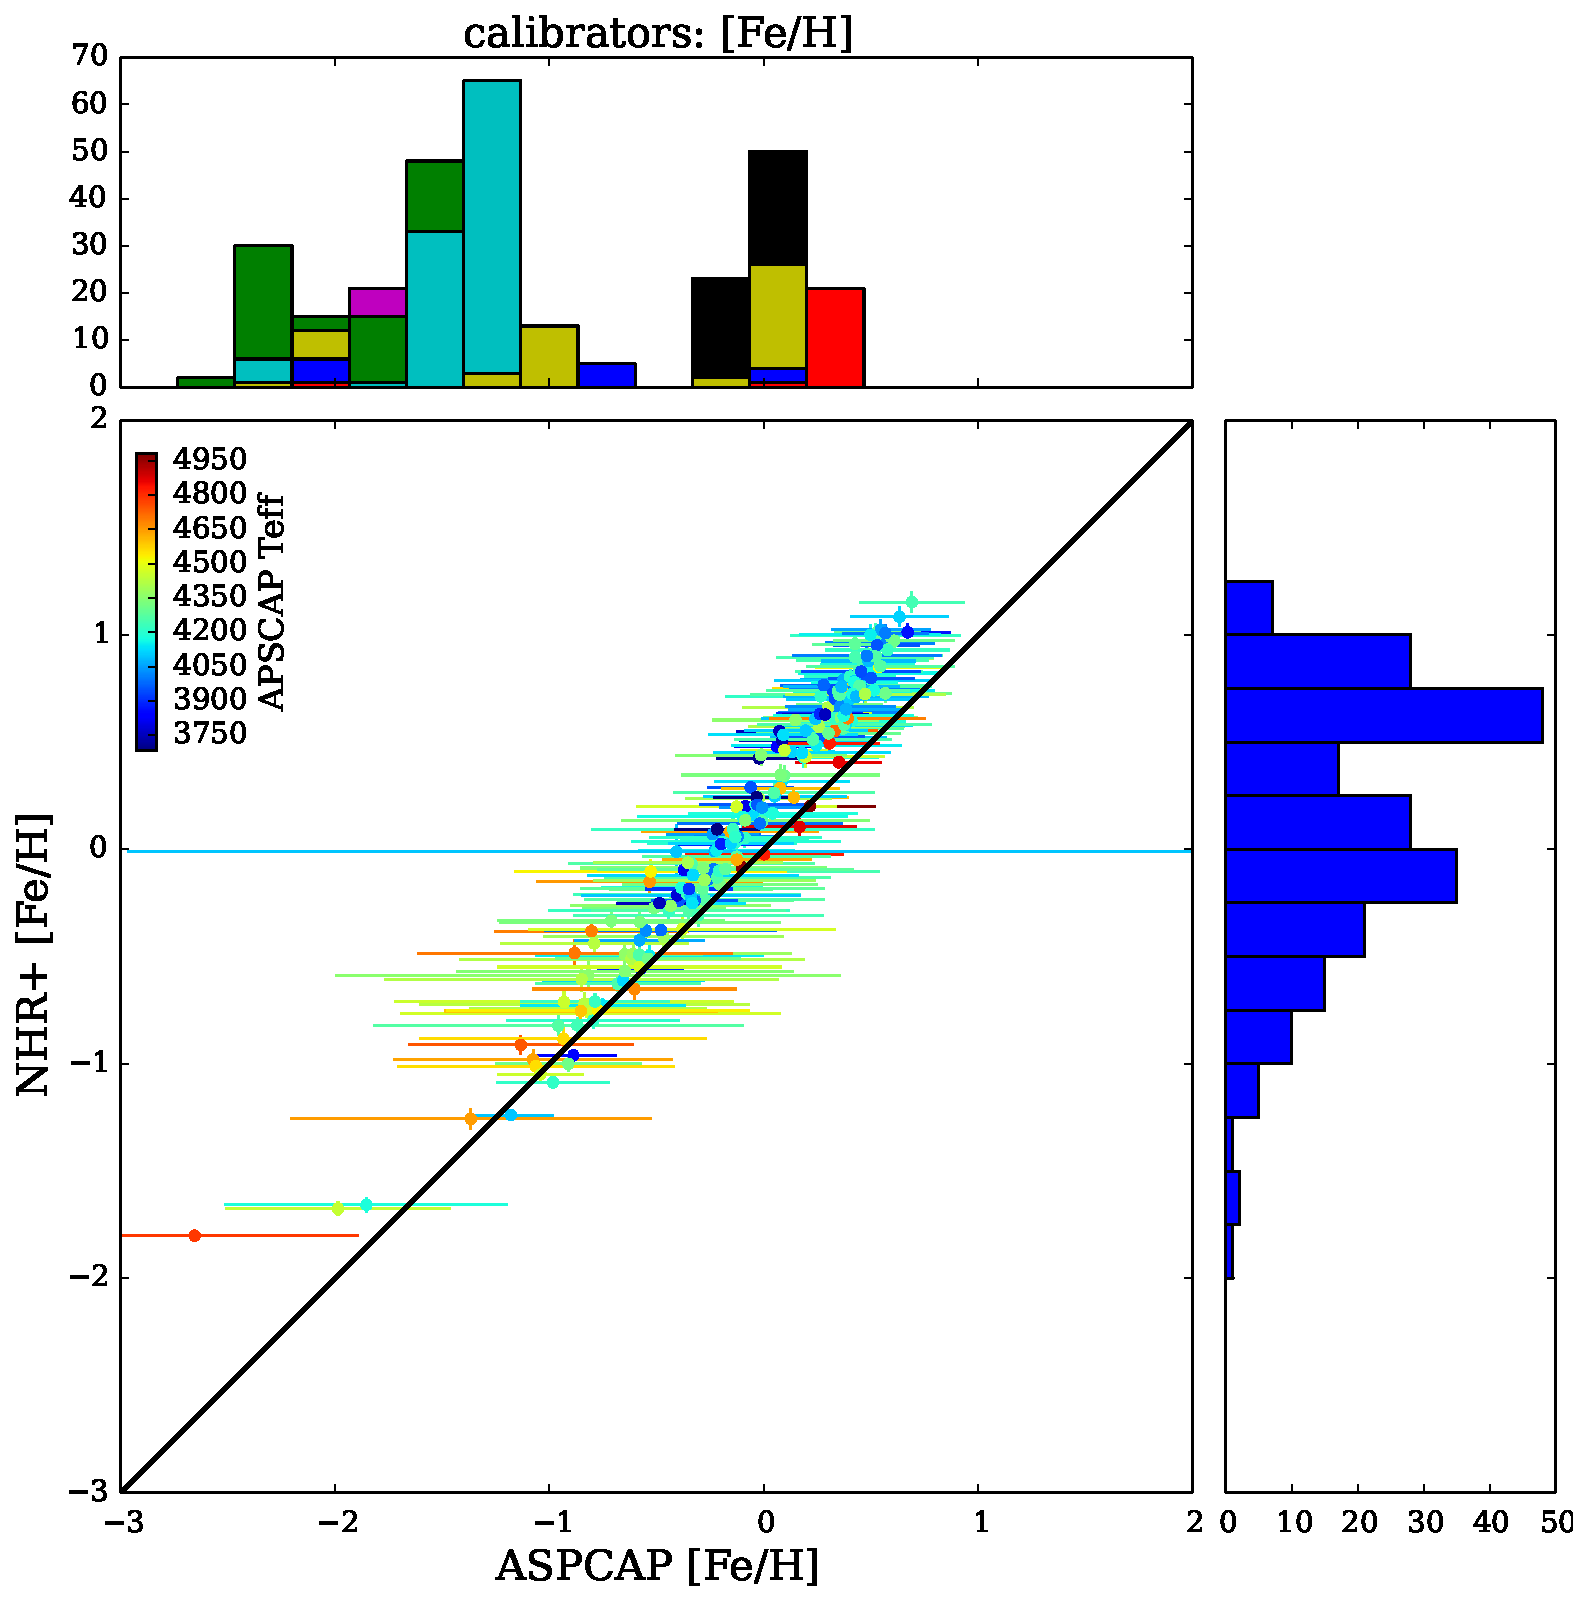
\includegraphics[width=\hsize]{./plots/cal_feh.eps}
\caption{\textbf{Need to change these to stack the histograms}: Showing the spread of calibration stars in training set across [Fe/H] - sparse sampling is not a problem in the centre for this label}
\label{fig:cal_feh}
\end{figure}

\begin{figure}[h!]
  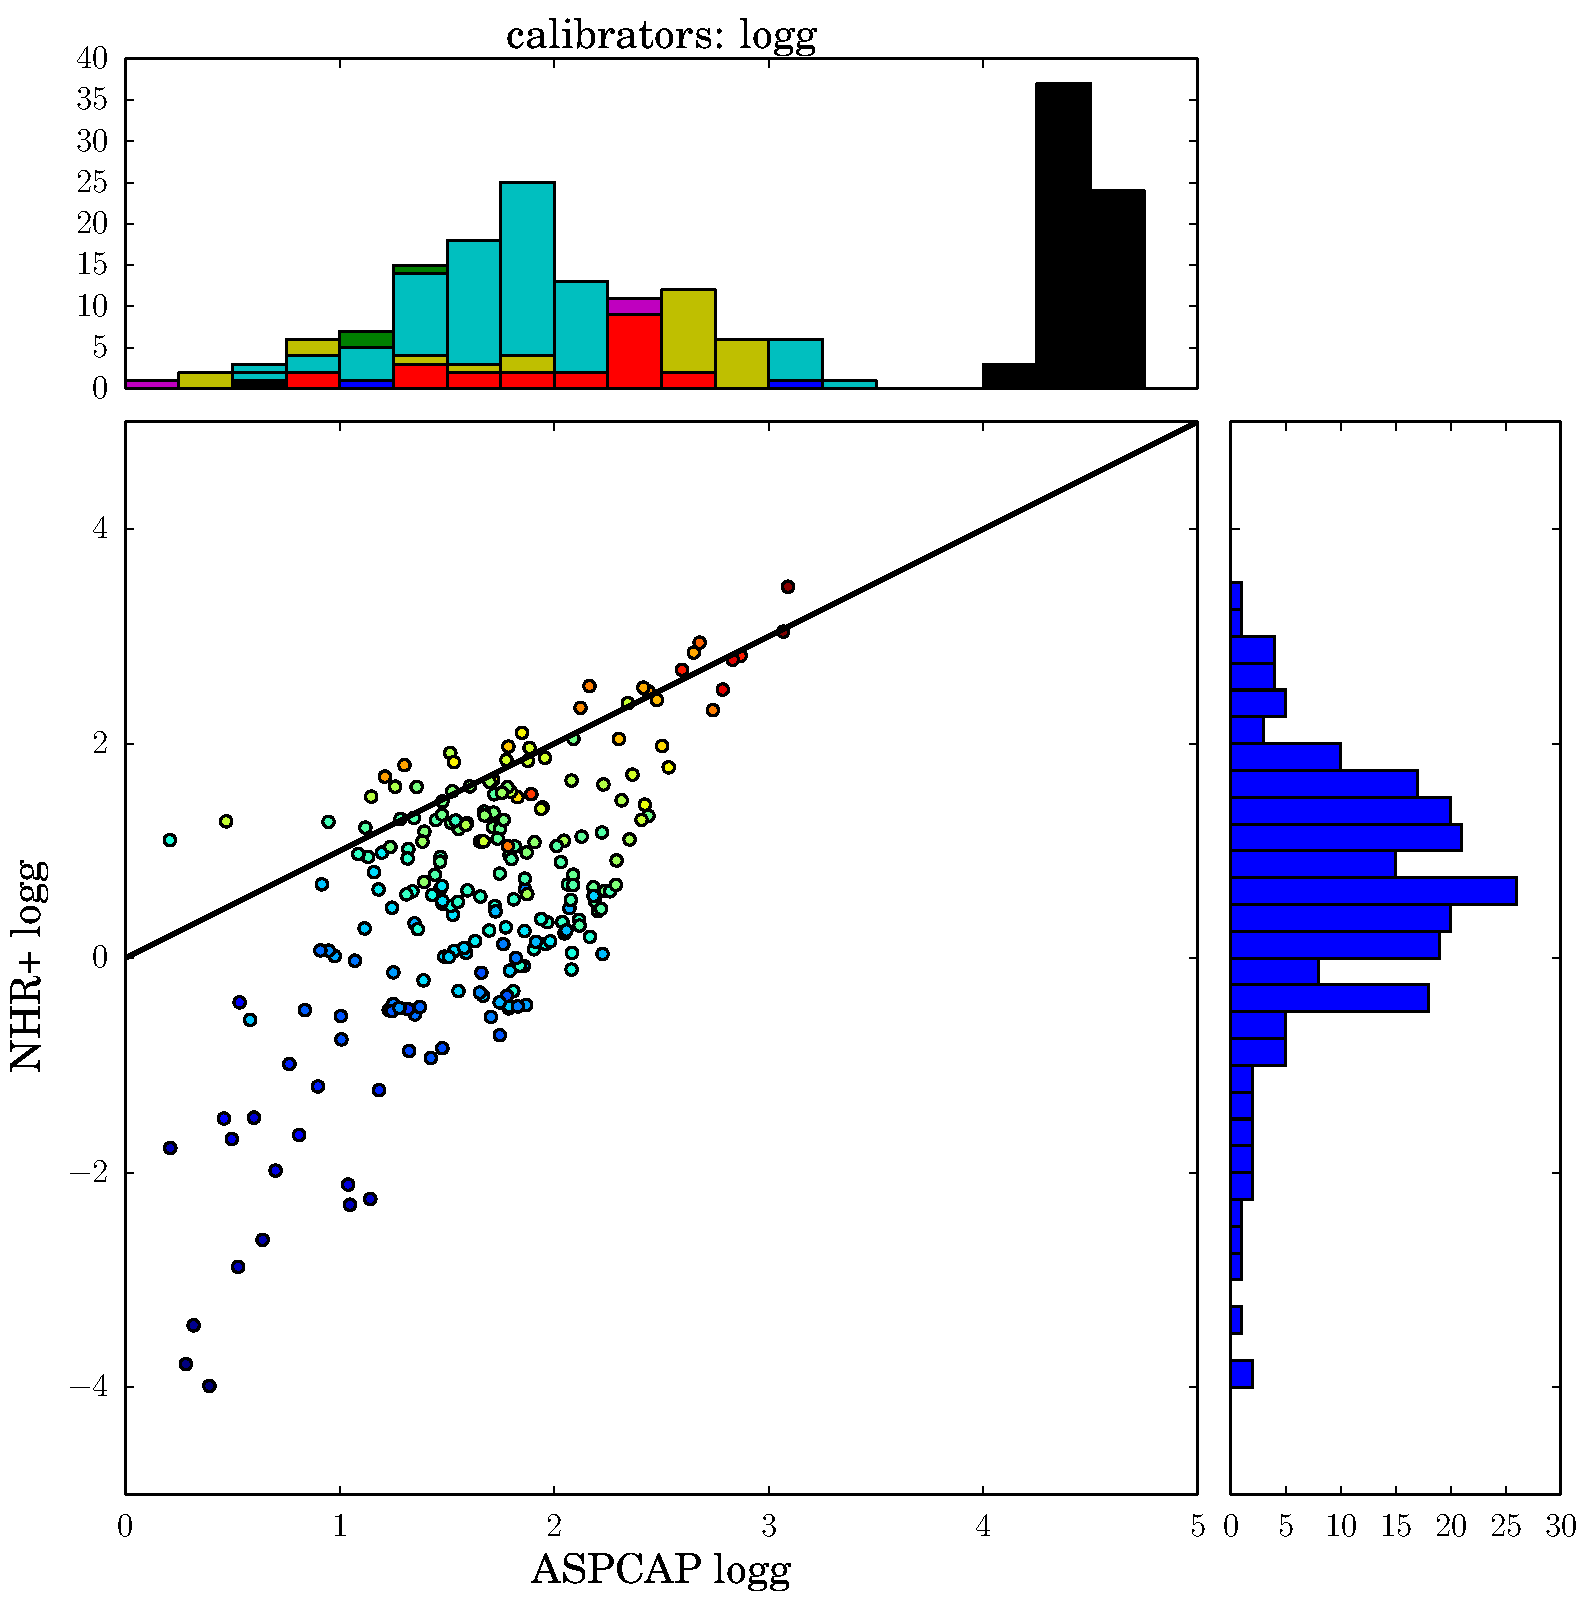
\includegraphics[width=\hsize]{./plots/cal_logg.eps}
\caption{Showing the spread of calibration stars in training set across log g ; missing sub giant stars - would be very good to have these }
\label{fig:cal_g}
\end{figure}

\begin{figure}[h!]
  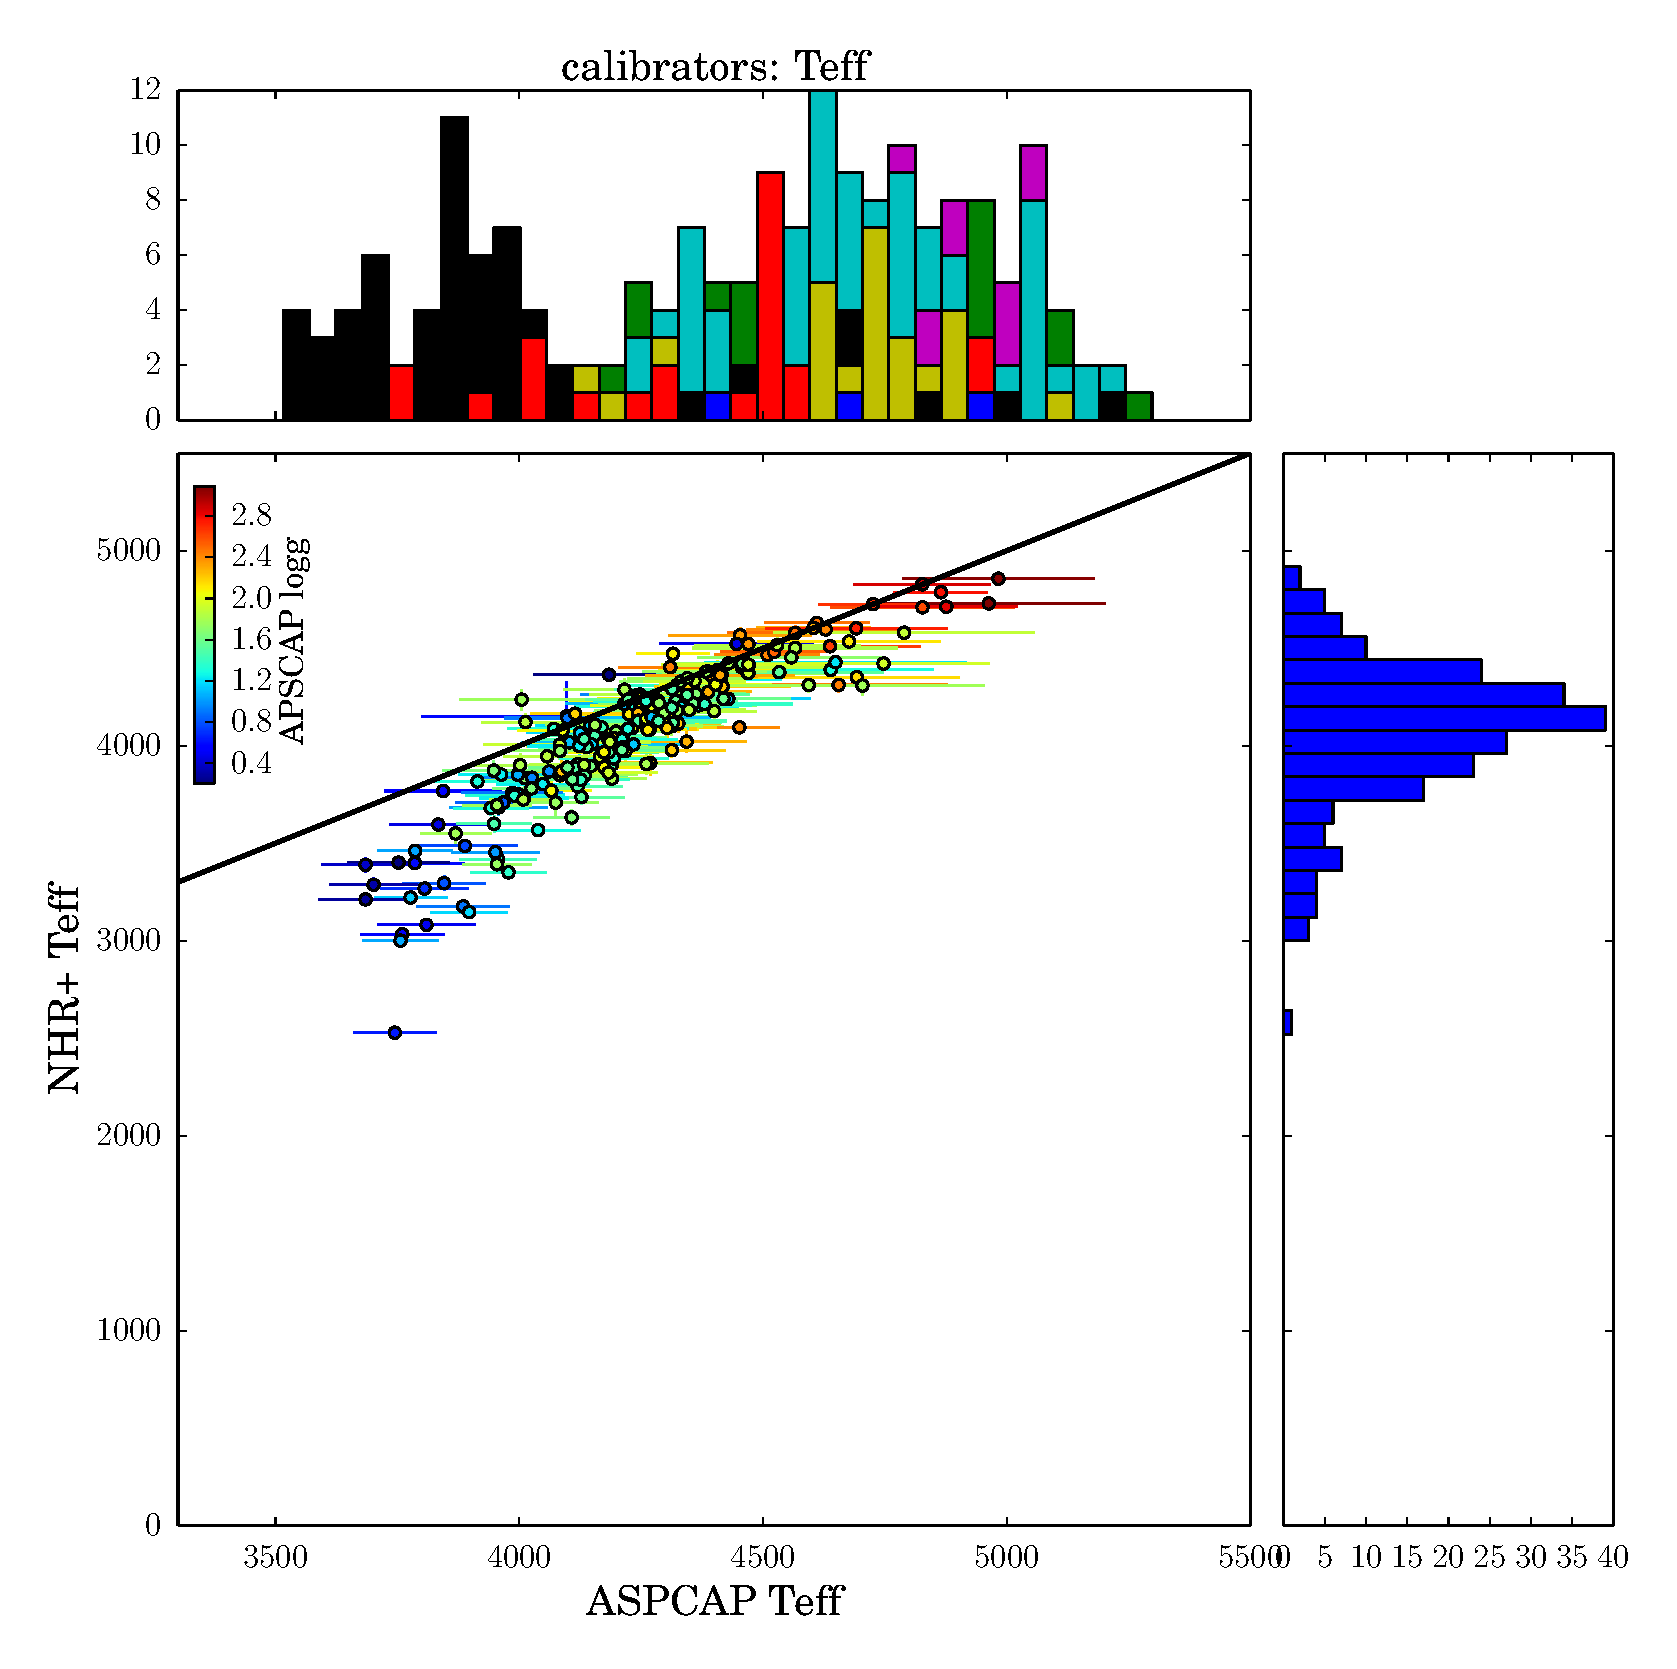
\includegraphics[width=\hsize]{./plots/cal_teff.eps}
\caption{Showing the spread of calibration stars in training set across Teff. Add error bars to these 3 figures showing the calibration.  put colourbar inside fig. have legend for the clusters as well.  }
\label{fig:cal_teff}
\end{figure}

\begin{figure}[h!]
  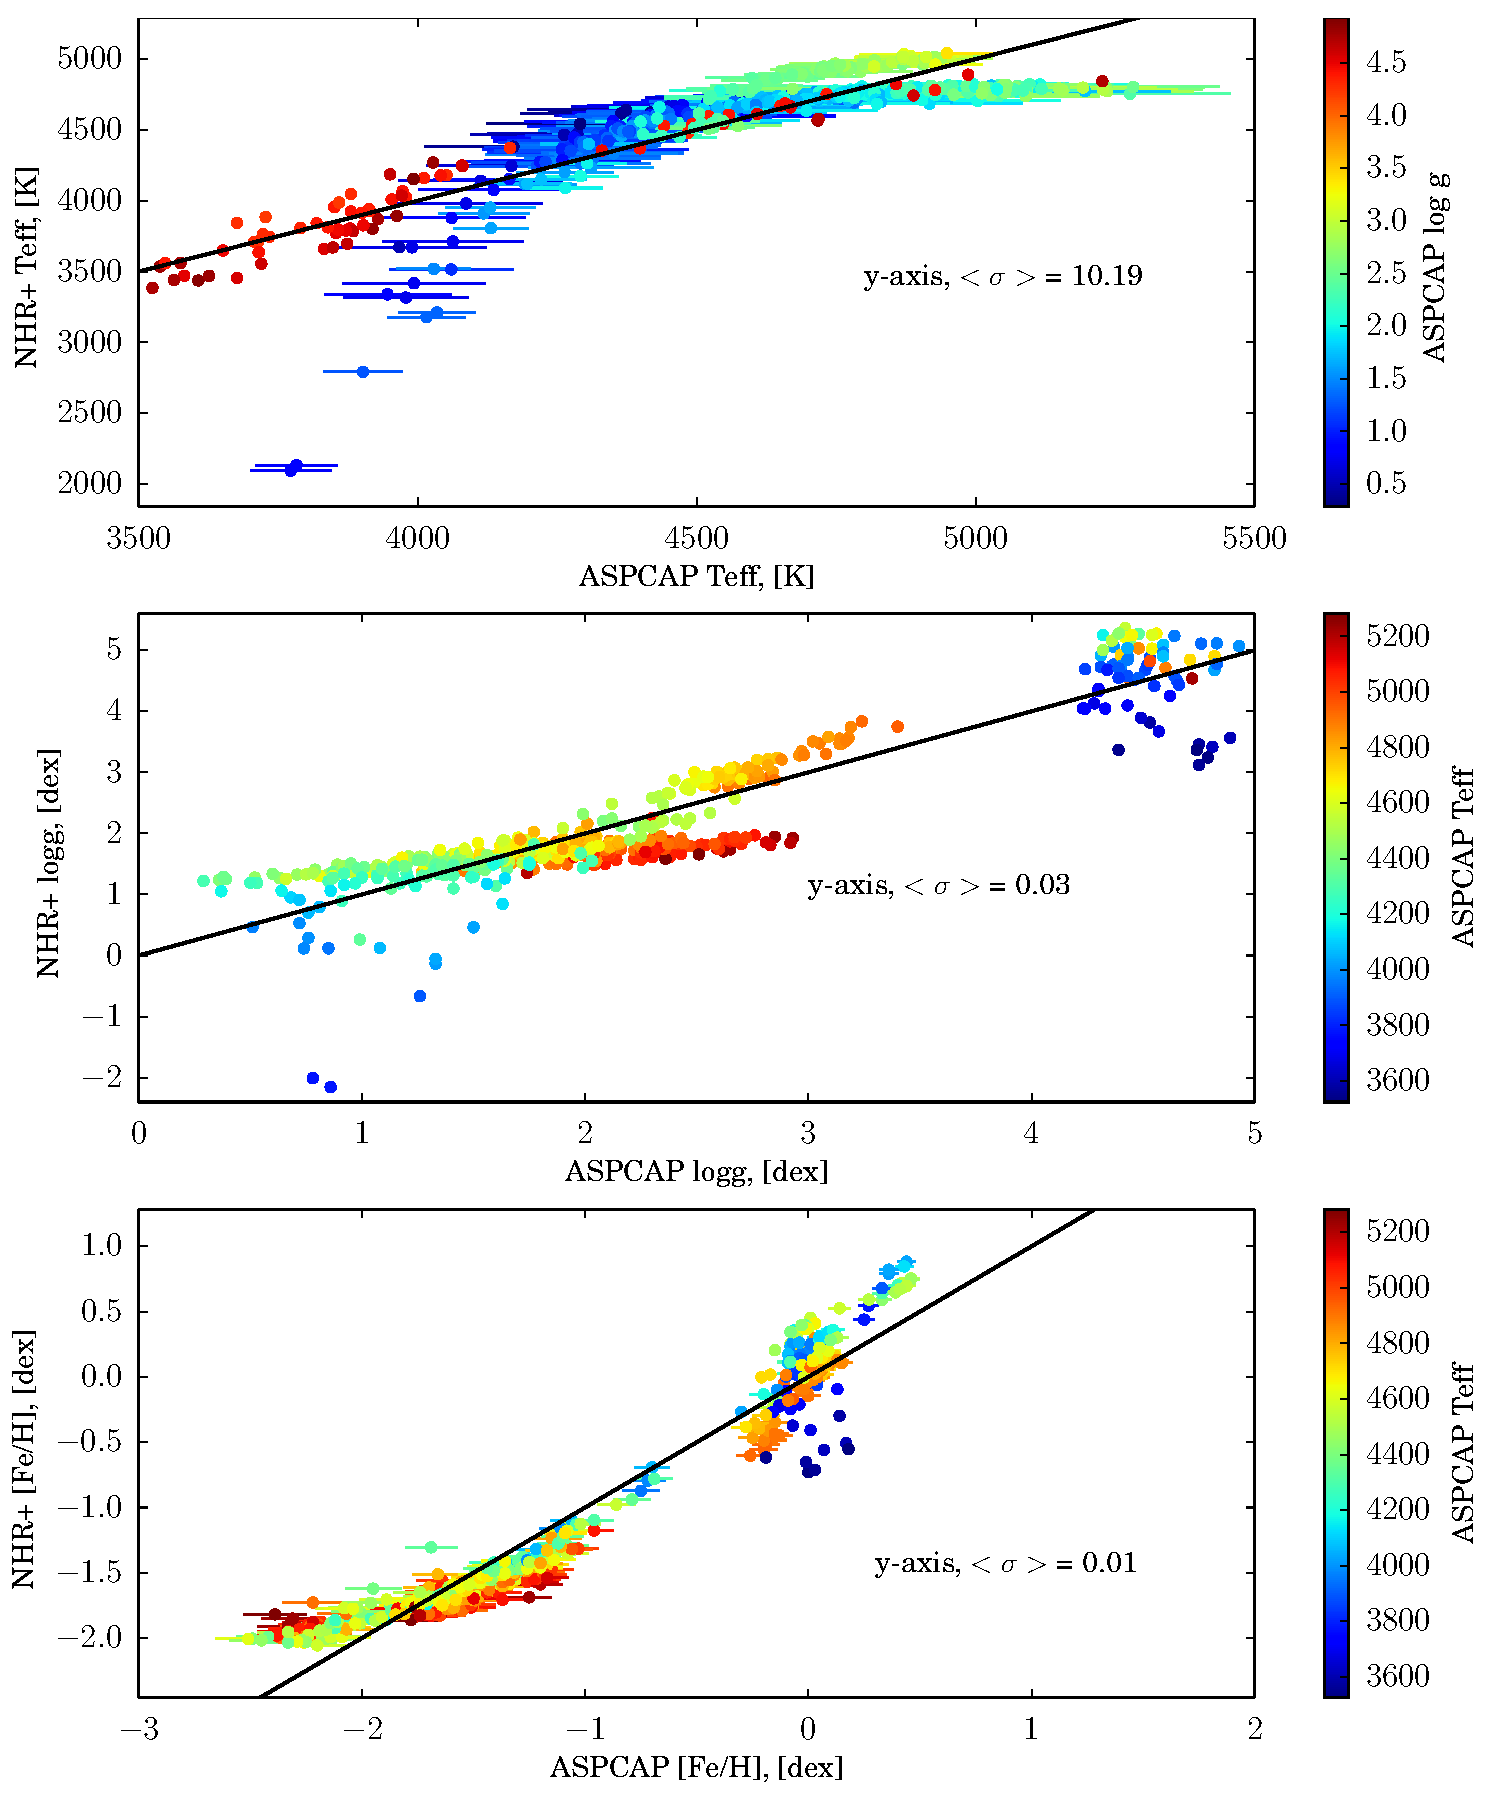
\includegraphics[width=\hsize]{./plots/fits_all3_self.eps}
\caption{this is not a cross validation this is the results of the training set run back through the code. }
\label{fig:cal_teff}
\end{figure}


\end{document}
